\documentclass[runningheads]{llncs}

\usepackage[T1]{fontenc}
\usepackage{lmodern}
\usepackage{graphicx}
\usepackage{float}
\usepackage{booktabs}
\usepackage{amsmath}
\usepackage{amssymb}
\usepackage{array}
\usepackage{multirow}
\usepackage[hidelinks]{hyperref}
\usepackage{xcolor}

\renewcommand\UrlFont{\color{blue}\rmfamily}

\begin{document}

\title{How Reliable Is Explainable AI for Plant Disease Recognition? A Robustness Evaluation under Real-World Image Transformations}

\titlerunning{Robustness of XAI for Plant Disease Recognition}

\author{Pham Tien Phuc\inst{1} \and
Vinoth Nageshwaran\inst{2} \and
Quan Thanh Tho\inst{3} \and
Duong Phu Bao\inst{3} \and
Ngo Trung Tin\inst{3} \and
Nguyen Huy\inst{3} \and
Duong Tan Phuc\inst{3} \and
Le Tran Anh Thuong\inst{3}}

\authorrunning{P. T. Phuc et al.}

\institute{FPT University, Can Tho, Vietnam \\
\email{phucpt10@fpt.edu.vn} \and
University of the Cumberlands, Williamsburg, KY, USA \\
\email{vnageshwaran41452@ucumberlands.edu} \and
Ho Chi Minh City University of Technology (HCMUT), VNU-HCM, Ho Chi Minh City, Vietnam \\
\email{\{qttho,bao.duongphu,tin.ngo2413506\}@hcmut.edu.vn} \\
\email{\{huy.nguyencseai,phuc.duongtan2901,thuong.lehcmutk24\}@hcmut.edu.vn}}

\maketitle

\begin{abstract}
Deep neural networks achieve near-perfect accuracy on benchmark plant-disease
image datasets, and post-hoc explanation methods such as Class Activation
Mapping (CAM) are increasingly used to justify their predictions to agronomists.
Yet field images are rarely pristine: they are blurred, rotated, unevenly lit,
and noisy. We ask whether the \emph{explanations} produced for such models remain
reliable when the input undergoes realistic, label-preserving transformations. We
introduce a reproducible benchmarking framework that couples a controlled image
perturbation protocol (Gaussian blur, rotation, brightness scaling and additive
noise) with two complementary axes of evaluation: prediction consistency and
explanation stability. Using the unaugmented, leaf-split PlantVillage colour
dataset and three ImageNet-pretrained backbones (ResNet-50 and EfficientNet-B0 for
the explanation analysis; ViT-B/16 for classification context), we evaluate the
CAM family (Grad-CAM, Grad-CAM++, Score-CAM, Eigen-CAM, Layer-CAM), quantifying
explanation stability with Pearson correlation, SSIM and top-$k$ IoU between the
(geometrically aligned) original and perturbed saliency maps, and complementing it
with deletion, insertion and average-drop faithfulness metrics. Statistical
significance is assessed with bootstrap confidence intervals and Holm-corrected
paired tests. Our study yields four findings that are hidden by accuracy alone:
(i) explanation stability varies strongly by perturbation --- brightness is almost
inert whereas blur and noise are highly disruptive; (ii) Layer-CAM,
Grad-CAM++ and Eigen-CAM are the most stable and Grad-CAM reliably the least
(Holm-corrected, pooled and in 16/24 per-transform tests), yet Grad-CAM is the most
faithful --- an explicit stability--faithfulness trade-off; (iii) sensitivity is
architecture-dependent, with ResNet-50 most vulnerable to noise and
EfficientNet-B0 most vulnerable to blur; and (iv) explanation fragility gets
\emph{worse}, not better, as the model approaches deployment accuracy: on a fully
fine-tuned 98.9\%-accurate model the gradient/score methods (Grad-CAM, Score-CAM)
degrade sharply while element-wise and principal-component maps stay robust. We frame deployment implications as
hypotheses for field validation and release the full protocol, code and raw
measurements to support reproducible robustness auditing of agricultural XAI.
\keywords{Explainable AI \and Robustness \and Class Activation Mapping \and Plant disease recognition \and Trustworthy machine learning \and Benchmarking}
\end{abstract}

%======================================================================
\section{Introduction}
%======================================================================
Automated plant disease recognition from leaf images is one of the most mature
applications of deep learning in precision agriculture. Convolutional and, more
recently, transformer architectures routinely exceed 99\% accuracy on curated
benchmarks and are being embedded in mobile diagnostic tools used by growers and
extension agents~\cite{mohanty2016plantvillage,ferentinos2018,too2019}. Because
an incorrect diagnosis can trigger unnecessary pesticide application or crop
loss, the deployment of such models in agronomy is increasingly gated on
\emph{trust}: a practitioner must be able to see \emph{why} the model reached its
conclusion. Explainable AI (XAI), and in particular saliency methods from the
Class Activation Mapping (CAM) family, has become the default vehicle for this
transparency, highlighting the leaf regions deemed responsible for a
prediction~\cite{zhou2016cam,selvaraju2020gradcam,arrieta2020xai}. The need for
interpretable and trustworthy models is not unique to agriculture: it recurs
wherever machine learning informs high-stakes decisions, from interpretable
strength prediction in materials science~\cite{nageshwaran2026interpretable} to
machine-learning-based medical image classification~\cite{nageshwaran2024braintumor},
where an opaque prediction is difficult to act upon.

A saliency map is only useful if it is \emph{reliable}, and two failure modes
matter: the prediction may change under innocuous input variation, or --- more
insidiously --- the prediction may stay correct while the \emph{explanation} shifts
to unrelated regions, silently invalidating the justification shown to the user.
Interpretations are known to be fragile to perturbation in generic vision
settings~\cite{ghorbani2019fragile,alvarez2018robustness,adebayo2018sanity}, yet
the plant-disease community has largely evaluated XAI qualitatively, on clean
laboratory images, without a statistically grounded protocol --- even though field
acquisitions are routinely degraded by blur, tilt, uneven lighting and noise.
Whether the explanations underpinning agronomic trust survive these everyday
transformations is, to our knowledge, open.

\smallskip
\noindent\textbf{Research questions.} We study two questions.
\emph{RQ1 (prediction consistency):} how much do label-preserving image
transformations degrade classification, and does this depend on the backbone?
\emph{RQ2 (explanation stability):} do CAM explanations remain spatially
consistent under the same transformations, how do CAM variants compare, and does
stability align with faithfulness?

\smallskip
\noindent\textbf{Contributions.}
\begin{itemize}
  \item A \emph{reproducible image-perturbation protocol} for auditing
  agricultural XAI, comprising geometric, photometric and noise-based
  transformations with a geometry-aware alignment step that makes original and
  perturbed saliency maps directly comparable.
  \item A \emph{benchmarking framework} that jointly measures prediction
  consistency and explanation stability (Pearson, SSIM, top-$k$ IoU) alongside
  established faithfulness metrics (deletion, insertion, average drop), with
  bootstrap confidence intervals and Holm-corrected significance testing.
  \item An \emph{empirical study} on the leaf-split PlantVillage colour dataset ---
  classification across three backbones, and the explanation analysis on the two
  CNNs (four CAM methods on both, Score-CAM on EfficientNet-B0) --- reporting
  \emph{honest} results including cases where methods lose. It surfaces effects that
  accuracy alone conceals (a stability--faithfulness trade-off and
  architecture-dependent sensitivity), and adds a fully fine-tuned validation.
  \item Two diagnostic controls on the deployment-accuracy model: a Score-CAM
  weighting collapse (with a candidate fix) and evidence that the most-recommended
  CAM variants become near-class-agnostic --- so stability must be read jointly with
  faithfulness.
  \item A public release of code, the exact evaluation manifests and all raw
  per-image measurements to enable exact reproduction and extension.
\end{itemize}

\noindent The remainder of the paper is organised as follows. Section~\ref{sec:rw}
reviews architectures, CAM methods and XAI evaluation. Section~\ref{sec:prob}
formalises the problem and Section~\ref{sec:method} details the framework.
Section~\ref{sec:exp} reports experiments and discussion, and
Section~\ref{sec:concl} concludes.

%======================================================================
\section{Related Work}\label{sec:rw}
%======================================================================
\noindent\textbf{From descriptors to deep architectures.}
Deep learning displaced hand-crafted descriptors for plant-disease recognition:
residual networks~\cite{he2016resnet}, EfficientNet's compound
scaling~\cite{tan2019efficientnet} and the Vision
Transformer~\cite{dosovitskiy2021vit} all report $>99\%$ accuracy on
PlantVillage and related corpora~\cite{mohanty2016plantvillage,ferentinos2018,too2019},
motivating a shift of attention from raw accuracy to reliability and explanation
quality.

\smallskip
\noindent\textbf{CAM-family explanations.}
CAM~\cite{zhou2016cam} localises class evidence via global-average-pooled feature
maps. Grad-CAM generalises it to arbitrary CNNs using gradients flowing into the
last convolutional layer~\cite{selvaraju2020gradcam}; Grad-CAM++ refines the
weighting with higher-order gradient terms for better multi-instance
localisation~\cite{chattopadhay2018gradcampp}; Score-CAM removes the gradient
dependency, weighting each activation map by the confidence it induces through a
forward pass~\cite{wang2020scorecam}; Eigen-CAM takes the leading principal
component of the activation maps and is gradient-free~\cite{muhammad2020eigencam};
and Layer-CAM re-weights activations element-wise to yield sharper, hierarchical
maps~\cite{jiang2021layercam}. Perturbation- and gradient-based attributions such
as RISE~\cite{petsiuk2018rise} form a complementary family; we focus on CAM
methods because they dominate agricultural XAI practice.

\smallskip
\noindent\textbf{Evaluating explanations.}
Explanation quality is assessed along \emph{faithfulness} (deletion/insertion
curves~\cite{petsiuk2018rise}, average drop~\cite{chattopadhay2018gradcampp}),
\emph{localisation}, and \emph{sanity} --- sensitivity to model and
data~\cite{adebayo2018sanity}; a separate line argues that \emph{robustness}
(similar inputs $\rightarrow$ similar explanations) is itself a desideratum that
many attributions violate~\cite{alvarez2018robustness,ghorbani2019fragile}, and
toolkits such as Quantus~\cite{hedstrom2023quantus} consolidate these metrics.
SSIM~\cite{wang2004ssim} naturally compares two saliency maps.

\smallskip
\noindent\textbf{Positioning.}
Most agricultural XAI studies remain qualitative and use controlled imagery,
leaving robustness under realistic acquisition largely
unquantified~\cite{hamdaoui2026review,arrieta2020xai}. We fill this gap with a
statistically grounded framework that measures \emph{both} prediction consistency
and explanation stability under a reproducible transformation protocol, reporting
faithfulness jointly so trade-offs are explicit.

%======================================================================
\section{Problem Formulation}\label{sec:prob}
%======================================================================
Let $f:\mathcal{X}\rightarrow\mathbb{R}^{C}$ be a trained classifier mapping an
image $x\in\mathcal{X}\subset\mathbb{R}^{3\times H\times W}$ to logits over $C$
classes, with predicted label $\hat{y}(x)=\arg\max_{c} f_c(x)$. A CAM explainer
$\Phi$ produces a saliency map $\Phi(f,x,c)\in[0,1]^{H\times W}$ for target class
$c$; we always explain the class predicted on the \emph{original} image,
$c=\hat{y}(x)$, so that stability is measured for a fixed concept. We note that the
methods differ in how strongly they depend on $c$: Grad-CAM, Grad-CAM++, Layer-CAM
and Score-CAM are class-conditional (through the class logit or its gradients),
whereas Eigen-CAM explains the leading principal component of the activation maps
and is effectively class-agnostic. For Eigen-CAM, ``stability of the explanation
for class~$c$'' therefore reduces to stability of the dominant activation subspace;
we retain it as a widely used gradient-free baseline and interpret its scores with
this caveat rather than as a like-for-like class-conditional comparison.

Let $\mathcal{T}=\{T_1,\dots,T_m\}$ be a set of label-preserving transformations
$T:\mathcal{X}\rightarrow\mathcal{X}$ (Section~\ref{sec:method}). For a
transformation $T$ we define two reliability notions.

\smallskip
\noindent\textbf{Prediction consistency.} For an evaluation set $S$,
\begin{equation}
\mathrm{PC}(T)=\frac{1}{|S|}\sum_{x\in S}\mathbb{1}\!\left[\hat{y}(T(x))=\hat{y}(x)\right],
\label{eq:pc}
\end{equation}
where $\mathbb{1}[\cdot]$ is the indicator function. We also report the drop in
macro-averaged $F_1$ between the clean and transformed sets.

\smallskip
\noindent\textbf{Explanation stability.} A geometric transformation moves salient
content, so a naive pixel-wise comparison of $\Phi(f,x,\hat{y})$ and
$\Phi(f,T(x),\hat{y})$ would conflate genuine instability with expected motion.
We therefore align the original map into the transformed frame with the same
geometric operation, $A_T(\cdot)$ ($A_T=T$ for rotation, identity for photometric
transforms), and restrict comparison to the valid region
$M_T$ (pixels defined after $A_T$). Writing $u=A_T(\Phi(f,x,\hat{y}))$ and
$v=\Phi(f,T(x),\hat{y})$, stability is quantified by three metrics over $M_T$:
Pearson correlation $r(u,v)$; structural similarity $\mathrm{SSIM}(u,v)$; and the
intersection-over-union of the top-$k$ salient pixels,
\begin{equation}
\mathrm{IoU}_k(u,v)=\frac{|B_k(u)\cap B_k(v)|}{|B_k(u)\cup B_k(v)|},\qquad
B_k(w)=\{p: w_p\ge Q_{1-k}(w)\},
\label{eq:iou}
\end{equation}
with $Q_{1-k}$ the $(1{-}k)$ quantile. We report $k=0.2$ (top quintile); a
sensitivity check over $k\in\{0.1,0.2,0.3\}$ leaves the IoU-based ordering unchanged
(Eigen-CAM $>$ Layer-CAM $>$ Grad-CAM++ $>$ Grad-CAM at every $k$ on
EfficientNet-B0; this is the IoU ordering, cf.\ the Pearson-based ranking in
Table~\ref{tab:stab}), so the threshold does not drive our conclusions. Higher values
indicate more stable explanations. Perfect stability gives $r=\mathrm{SSIM}=\mathrm{IoU}_k=1$.

\smallskip
\noindent\textbf{Faithfulness.} Independently of transformations, we assess how
well $\Phi$ reflects $f$ on the clean image via deletion and insertion
AUC~\cite{petsiuk2018rise} and average drop~\cite{chattopadhay2018gradcampp}
(Section~\ref{sec:method}). Reliability requires stability \emph{and}
faithfulness; the framework reports both so trade-offs are visible.

%======================================================================
\section{Evaluation Framework}\label{sec:method}
%======================================================================
\noindent\textbf{Dataset.} We use the PlantVillage colour configuration obtained
programmatically from the official \texttt{mohanty/PlantVillage} Hugging Face
repository. We adopt the repository's \emph{leaf-based} train/test split, which
groups all views of a physical leaf on one side of the split and thereby prevents
leakage between near-duplicate images. To keep the study executable at CPU scale
we draw a class-balanced subset with a fixed seed: 35 training and 25 test images
per class across all 38 \{crop, condition\} classes (1{,}330 train / 950 test
images). Images are resized to $160\times160$ (CNNs) and normalised with ImageNet
statistics.

\smallskip
\noindent\textbf{Backbones and training.} We evaluate three ImageNet-pretrained
backbones: ResNet-50~\cite{he2016resnet}, EfficientNet-B0~\cite{tan2019efficientnet}
and ViT-B/16~\cite{dosovitskiy2021vit} (ViT uses its native $224\times224$
input). Given the memory budget we adopt \emph{linear probing}: backbone weights
are frozen and a linear classification head is trained on the pooled features
(global-average-pooled last convolutional map for CNNs; the class token for ViT)
using Adam. Freezing the backbone does not affect CAM computation, which
back-propagates through the frozen convolutional stack to the target layer.

\smallskip
\noindent\textbf{Transformation protocol.} Four label-preserving transformations
model common field degradations, applied to the $[0,1]$ image before
normalisation: \emph{Gaussian blur} ($9\times9$ kernel, $\sigma=2$),
\emph{rotation} ($+15^{\circ}$, bilinear), \emph{brightness} scaling
($\times1.3$, clipped) and additive \emph{Gaussian noise} ($\sigma=0.08$). The
identity transform serves as reference.

\smallskip
\noindent\textbf{CAM methods.} We evaluate Grad-CAM, Grad-CAM++, Eigen-CAM and
Layer-CAM on both CNN backbones, and additionally Score-CAM on EfficientNet-B0.
Score-CAM performs one forward pass per activation channel (1{,}280 for
EfficientNet-B0, 2{,}048 for ResNet-50); on CPU this is roughly $50$--$90\times$
slower than the gradient methods, so we restrict it to EfficientNet-B0 on a
$12$-image subset and report it with its own sample size. All maps are computed
with a public CAM library~\cite{gildenblat2021pytorchcam} on the last
convolutional block.

\smallskip
\noindent\textbf{Evaluation sets.} Prediction consistency (Eq.~\ref{eq:pc}) is
measured on a $190$-image set (5 per class). Explanation stability and
faithfulness are measured on a $38$-image set (one image per class that is
correctly classified on the \emph{clean} input, shared across backbones); this
smaller set reflects the cost of computing five CAMs under five conditions per
image and is reflected in the reported confidence intervals. A transformation may
flip the prediction; because we always explain the clean predicted class $c$, such
an image is \emph{not} removed from the stability computation --- the case in which
the prediction changes (or, worse, stays correct while the map migrates) is exactly
the failure mode we wish to capture. Prediction-level effects are reported
separately in Section~5.2.

\smallskip
\noindent\textbf{Faithfulness computation.} Deletion progressively zeroes the most
salient pixels (low AUC is better); insertion progressively reveals them from a
blurred baseline (high AUC is better); both use 20 steps. Average drop is
$\max(0, p_{\text{full}}-p_{\text{mask}})/p_{\text{full}}\times100$, where
$p_{\text{mask}}$ uses the CAM as a soft mask (lower is better).

\smallskip
\noindent\textbf{Statistics.} We compute bootstrap $95\%$ CIs ($2{,}000$ resamples)
for all means; to respect the page limit they are printed in Tables~\ref{tab:stab}
and~\ref{tab:ft} and in the released records for the rest. Pairwise comparisons use
per-image mean Pearson stability with Wilcoxon signed-rank tests and Holm correction
within each backbone~\cite{holm1979}.

%======================================================================
\section{Experiments and Results}\label{sec:exp}
%======================================================================
\noindent\textbf{Implementation.} All experiments run on CPU (4 cores, PyTorch).
Seeds are fixed ($42$) throughout; the released code reproduces every table and
figure from the saved per-image records.

\subsection{Classification performance}
Under linear probing on the 38-class task (950 test images), clean accuracy /
macro-$F_1$ is $0.868/0.867$ (ResNet-50), $0.883/0.882$ (EfficientNet-B0) and
$0.919/0.918$ (ViT-B/16). These are below the near-saturated numbers usually quoted
for PlantVillage --- because we freeze the backbone and subsample --- but are more
than sufficient as a substrate for a relative robustness study (\S5.6 revisits this
with a fully fine-tuned 98.9\% model).

\subsection{RQ1: Prediction consistency under transformation}
Table~\ref{tab:pred} quantifies prediction robustness.
Brightness scaling is almost inert (prediction consistency $\mathrm{PC}=0.95$ for
both backbones; macro-$F_1$ essentially unchanged). Rotation causes a moderate
drop ($\mathrm{PC}=0.83$ for ResNet-50, $0.77$ for EfficientNet-B0). Blur and
noise are the most damaging, but the ranking is architecture-dependent:
ResNet-50 is most harmed by noise ($\mathrm{PC}=0.53$, macro-$F_1$ $-0.37$)
whereas EfficientNet-B0 is most harmed by blur ($\mathrm{PC}=0.53$, macro-$F_1$
$-0.38$). Thus even at the prediction level, robustness is not a property of the
task alone but of the model, a distinction that a single clean-accuracy number
hides.

\begin{table}[t]
\centering
\caption{Prediction consistency (PC, Eq.~\ref{eq:pc}) and macro-$F_1$ drop
relative to clean, per transformation (190-image set).}
\label{tab:pred}
\begin{tabular}{lcccc}
\toprule
 & \multicolumn{2}{c}{ResNet-50} & \multicolumn{2}{c}{EfficientNet-B0} \\
\cmidrule(lr){2-3}\cmidrule(lr){4-5}
Transform & PC & $\Delta F_1$ & PC & $\Delta F_1$ \\
\midrule
Blur       & 0.621 & $-0.283$ & 0.532 & $-0.375$ \\
Rotate     & 0.832 & $-0.086$ & 0.774 & $-0.127$ \\
Brightness & 0.947 & $+0.008$ & 0.947 & $-0.007$ \\
Noise      & 0.532 & $-0.372$ & 0.695 & $-0.212$ \\
\bottomrule
\end{tabular}
\end{table}


\subsection{RQ2: Explanation stability}
Table~\ref{tab:stab} summarises stability, averaged over transforms
(per-transform values in Appendix~A). The picture mirrors RQ1: brightness leaves
explanations almost untouched ($r>0.95$), while blur and noise dominate
instability. \textbf{Layer-CAM} and \textbf{Grad-CAM++} are the most stable
($r\!=\!0.88$/$0.87$), \textbf{Grad-CAM} consistently the least ($r\!=\!0.77$).
Eigen-CAM is competitive on ResNet-50 ($r\!=\!0.87$) but degrades under rotation on
EfficientNet-B0 ($r\!=\!0.67$); Score-CAM is already the least stable under blur
($r\!=\!0.39$, wide CI, small sample), foreshadowing its fine-tuned collapse in
\S5.6 (Eigen-CAM, by contrast, remains the \emph{most} stable there).

\begin{table}[t]
\centering
\caption{Explanation stability averaged over the four transformations (mean with
bootstrap 95\% CI; higher is better). $n{=}38$ except Score-CAM ($n{=}12$). The
wide, overlapping CIs are consistent with the significance analysis: methods are
\emph{ordered} but individual per-transform differences are not powered at $n{=}38$.}
\label{tab:stab}
\resizebox{\textwidth}{!}{%
\begin{tabular}{llccc}
\toprule
Backbone & Method & Pearson $r$ & SSIM & IoU$_{0.2}$ \\
\midrule
\multirow{4}{*}{ResNet-50}
 & Grad-CAM   & 0.769 [0.722,0.813] & 0.673 [0.644,0.700] & 0.561 [0.518,0.601] \\
 & Grad-CAM++ & 0.879 [0.853,0.900] & 0.806 [0.789,0.821] & 0.632 [0.593,0.670] \\
 & Eigen-CAM  & 0.873 [0.832,0.907] & 0.789 [0.757,0.817] & 0.697 [0.657,0.737] \\
 & Layer-CAM  & \textbf{0.882} [0.857,0.904] & \textbf{0.809} [0.793,0.824] & 0.637 [0.598,0.674] \\
\midrule
\multirow{5}{*}{EfficientNet-B0}
 & Grad-CAM   & 0.771 [0.704,0.831] & 0.788 [0.758,0.815] & 0.604 [0.552,0.653] \\
 & Grad-CAM++ & 0.872 [0.828,0.909] & 0.796 [0.771,0.818] & 0.689 [0.638,0.733] \\
 & Eigen-CAM  & 0.824 [0.738,0.897] & \textbf{0.802} [0.754,0.846] & \textbf{0.724} [0.659,0.782] \\
 & Layer-CAM  & \textbf{0.873} [0.833,0.909] & 0.799 [0.774,0.822] & 0.690 [0.643,0.731] \\
 & Score-CAM  & 0.761 [0.672,0.842] & 0.727 [0.675,0.783] & 0.596 [0.500,0.692] \\
\bottomrule
\end{tabular}}
\end{table}


\noindent\textbf{Significance.} On the pooled score (per-image Pearson averaged
over the four transformations), Holm-corrected Wilcoxon tests find Grad-CAM
significantly less stable than Grad-CAM++, Eigen-CAM and Layer-CAM on ResNet-50
(all $p_{\text{Holm}}<10^{-3}$) and than Grad-CAM++ and Layer-CAM on
EfficientNet-B0 ($p_{\text{Holm}}=0.014$). The effect also holds
\emph{per transformation}: of the 24 Grad-CAM-vs-other comparisons (2 backbones
$\times$ 4 transforms $\times$ 3 pairs, Score-CAM excluded; full table in
Appendix~A), Grad-CAM is significantly less stable in 16 ($p_{\text{Holm}}<0.05$),
most robustly under noise and blur
($p_{\text{Holm}}<10^{-3}$); it is not significant only under brightness (where all
methods are near-ceiling) and for a few rotation pairs (per-transform table in the
released records). Differences among the top three methods are small --- the
near-identical Grad-CAM++/Layer-CAM pair can reach significance on negligible
($<0.01$) gaps, which we do not interpret substantively --- so we treat Layer-CAM,
Grad-CAM++ and Eigen-CAM as jointly most stable and Grad-CAM as reliably least.

\subsection{Faithfulness and the stability--faithfulness trade-off}
Table~\ref{tab:faith} reports faithfulness. Strikingly, the ranking partly
inverts that of stability. On EfficientNet-B0, \textbf{Grad-CAM} attains by far
the best average drop ($19.9$ vs.\ $45$--$66$ for the others) and a competitive
deletion AUC, i.e.\ the very method that is \emph{least stable} is among the
\emph{most faithful} to the model on clean inputs. Score-CAM achieves the best
insertion AUC ($0.70$). This trade-off has a practical reading: a method that
hugs the model's decision surface tightly (faithful) can also track spurious,
perturbation-induced fluctuations (unstable), whereas smoother maps (Layer-CAM,
Grad-CAM++) are more stable but less sharply tied to the logit. Reliability
assessments that optimise only one axis are therefore misleading; both must be
reported.

\begin{table}[t]
\centering
\small
\setlength{\tabcolsep}{5pt}
\caption{Faithfulness on clean images (mean; 95\% CIs in the released records).
Deletion$\downarrow$, Insertion$\uparrow$, Average drop (\%)$\downarrow$.
$n{=}38$ except Score-CAM ($n{=}12$).}
\label{tab:faith}
\begin{tabular}{llccc}
\toprule
Backbone & Method & Deletion & Insertion & Avg.\ drop \\
\midrule
\multirow{4}{*}{ResNet-50}
 & Grad-CAM   & 0.363 & 0.559 & \textbf{35.6} \\
 & Grad-CAM++ & 0.393 & 0.558 & 36.9 \\
 & Eigen-CAM  & 0.399 & \textbf{0.562} & 57.8 \\
 & Layer-CAM  & 0.391 & 0.559 & 36.9 \\
\midrule
\multirow{5}{*}{EfficientNet-B0}
 & Grad-CAM   & 0.195 & 0.626 & \textbf{19.9} \\
 & Grad-CAM++ & 0.187 & 0.621 & 45.6 \\
 & Eigen-CAM  & 0.212 & 0.611 & 66.5 \\
 & Layer-CAM  & \textbf{0.183} & 0.622 & 45.1 \\
 & Score-CAM  & 0.214 & \textbf{0.701} & 37.9 \\
\bottomrule
\end{tabular}
\end{table}

\subsection{Qualitative analysis}
Figure~\ref{fig:qual} shows a low-stability case: for a diseased corn leaf (common
rust) whose prediction is preserved, the heatmaps migrate substantially under blur,
rotation and noise --- drifting off the visible rust pustules --- while remaining
nearly fixed under brightness. This is exactly the insidious failure mode motivating
the study: the label is right, but the explanation no longer coincides with the
disease evidence it highlighted on the clean image. High-stability-quantile cases
(released records) instead show near-identical maps across all conditions, so
instability is concentrated in a subset of images and perturbations, not uniform.

\begin{figure}[t]
\centering
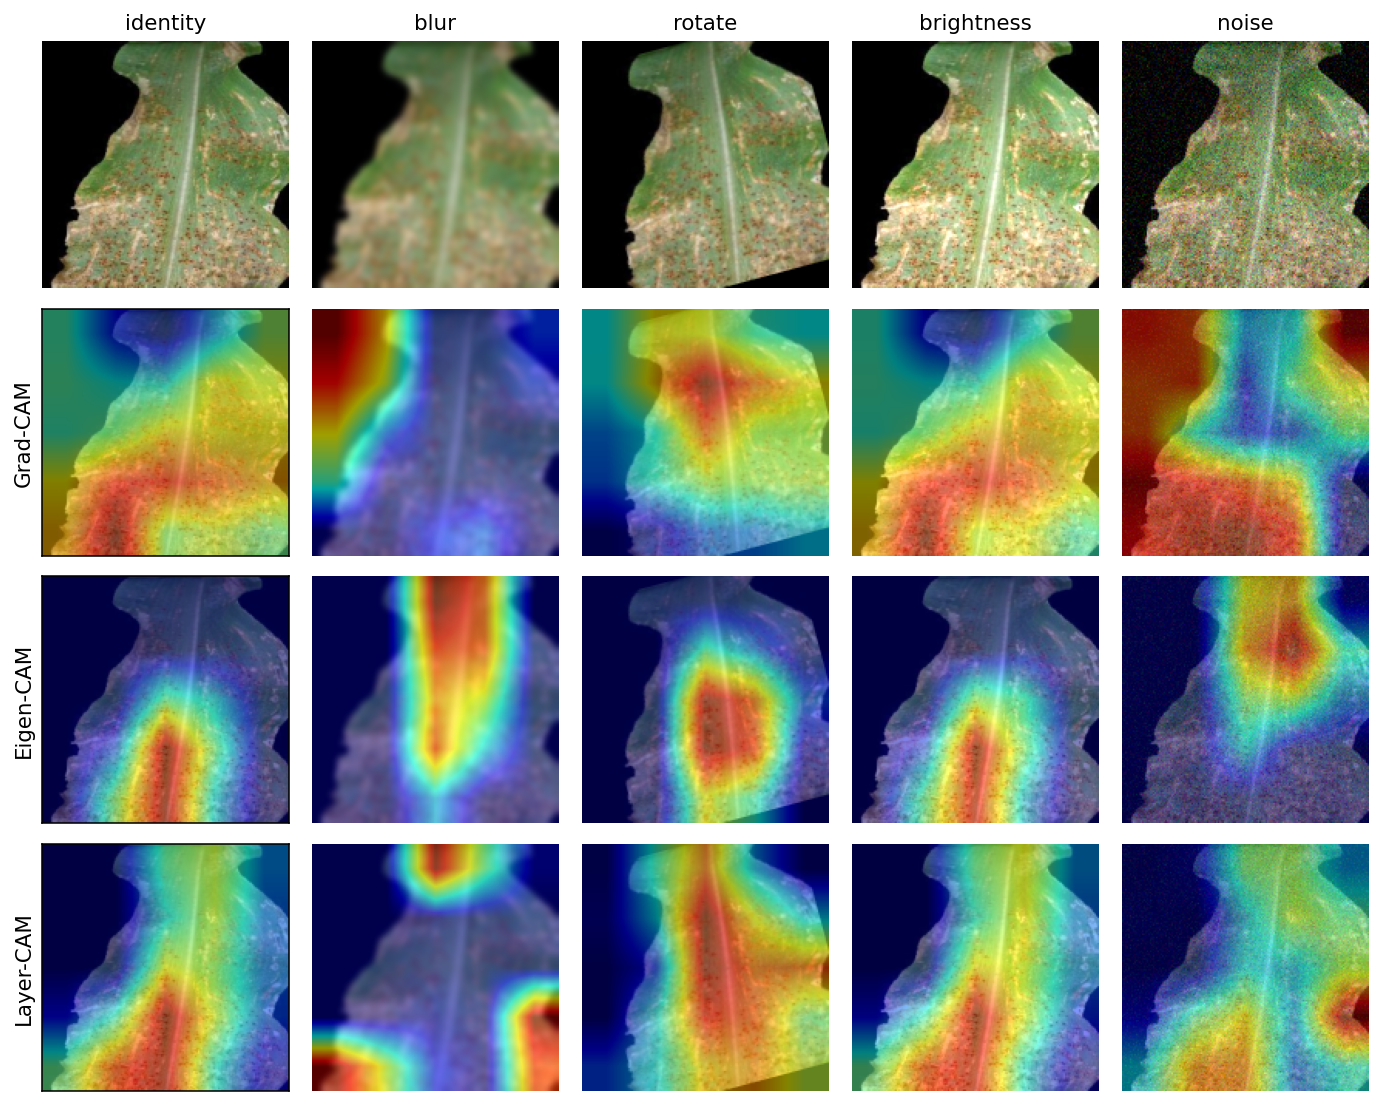
\includegraphics[width=0.72\textwidth]{figures/fig_qual_compact.png}
\caption{A low-stability example on a \emph{diseased} leaf (EfficientNet-B0, corn
common rust; rust pustules visible across the lamina). Rows: representative CAM
methods; columns: identity and the four transforms (Grad-CAM++ and Score-CAM
behave similarly; full 5-method montage in the released records). The prediction is
preserved, yet the heatmaps migrate markedly under blur, rotation and noise ---
drifting off the lesion-bearing regions --- while brightness is benign.}
\label{fig:qual}
\end{figure}

\subsection{Fine-tuned validation and two controls}
To test whether the frozen-backbone findings persist once features specialise to
disease cues, we fully fine-tuned EfficientNet-B0 end-to-end; it reaches
\textbf{98.9\%} accuracy / macro-$F_1$ --- the near-saturated regime of deployed
models, up from 88.3\% for the linear probe. Re-running the protocol on the
\emph{same} 38 images (paired comparison, Table~\ref{tab:ft}) shows the
stable-method ranking transfers --- Eigen-CAM, Layer-CAM and Grad-CAM++ stay high
($r\approx0.79$--$0.83$) --- while Grad-CAM roughly halves ($0.77\!\to\!0.39$; on a
larger $n{=}100$ set it falls to $0.20$). Fine-tuning thus makes gradient-weighted
maps more brittle, not less: explanation fragility \emph{worsens} as the model
approaches deployment accuracy.

\noindent\textbf{Control 1 --- the Score-CAM collapse is a property of the
published method, not a bug.} On the fine-tuned model Score-CAM falls to
$r\!=\!0.04$ ($n{=}100$). The cause is the weighting that the original Score-CAM
formulation \emph{specifies}: channels are weighted by a softmax over their
per-channel target \emph{logits}. On the confident model this distribution peaks
sharply --- its entropy drops from $6.25$ to $2.16$ (max $7.15$) and a single
channel captures $53\%$ of the weight (vs.\ $1\%$ frozen) --- so the map collapses
onto one volatile channel. As a \emph{proposed modification}, replacing the softmax
with a bounded min--max channel weighting more than doubles stability on a small
diagnostic set ($4$ easier images, hence a higher $0.28$ baseline than the $n{=}100$
headline of $0.04$): mean Pearson rises $0.28\!\to\!0.64$. Since the target is
already the pre-softmax logit, this is distinct from classic softmax-gradient
saturation; a full-scale evaluation is future work.

\noindent\textbf{Control 2 --- stability can be inflated by class-insensitivity.}
The fine-tuned stability ``winners'' are exactly the methods that barely depend on
the predicted class. Measuring class-sensitivity as $1-r$ between a method's map for
the predicted class and for a single random non-predicted class (one draw per image,
seed $42$; Table~\ref{tab:ft}, last column), the three methods with near-zero
class-sensitivity (Eigen-CAM $0.00$, Grad-CAM++ $0.03$, Layer-CAM $0.02$) are
precisely the three that stay stable, while the one strongly class-conditional method
(Grad-CAM, $0.97$) is the one that collapses. This is not an artefact of Grad-CAM's
own instability: a self-consistency control --- $1-r$ between a method's map on the
image and on a jittered copy of the \emph{same} class ($\sigma{=}0.02$ Gaussian) ---
is $\approx0.01$ for \emph{every} method, Grad-CAM included. Grad-CAM's maps are thus
self-consistent under input noise yet change almost completely when the target class
changes ($0.01$ vs.\ $0.97$), so its high class-sensitivity is genuine
class-discrimination; the other methods' near-zero values are genuine
class-\emph{agnosticism}, not measurement noise. A map that
scarcely moves when the target class changes also has little reason to move under
perturbation, so \emph{stability alone can be inflated by uninformative
explanations} --- which is exactly why our framework reads stability jointly with
faithfulness (Table~\ref{tab:faithpert}) rather than in isolation.

\noindent Beyond our metric, this is a finding about the \emph{methods}. Grad-CAM++
and Layer-CAM are class-conditional \emph{by construction}, yet on the model closest
to deployment their maps barely change when a random target class is substituted ---
a failure of the model-and-data sensitivity that saliency sanity checks
demand~\cite{adebayo2018sanity}. In other words, at deployment-level accuracy the
CAM variants most recommended in the agricultural literature can produce
near-class-agnostic explanations; accuracy conceals this, and stability alone would
have rewarded it.

\begin{table}[t]
\centering
\caption{Frozen (linear-probe) vs.\ fully fine-tuned EfficientNet-B0 on the
\emph{same} 38 images: explanation stability (Pearson $r$, mean [95\% CI]) and
class-sensitivity (higher $=$ more class-conditional; see Control~2). Score-CAM is
treated separately in Control~1. The three near-class-agnostic methods are the
three that stay stable; the strongly class-conditional method (Grad-CAM) collapses.}
\label{tab:ft}
\resizebox{\textwidth}{!}{%
\begin{tabular}{lccc}
\toprule
Method & Frozen $r$ & Fine-tuned $r$ (98.9\% acc.) & Class-sensitivity \\
\midrule
Grad-CAM   & 0.771 [0.704,0.831] & 0.392 [0.313,0.475] & 0.97 \\
Grad-CAM++ & 0.872 [0.828,0.909] & 0.808 [0.777,0.840] & 0.03 \\
Eigen-CAM  & 0.824 [0.738,0.897] & \textbf{0.828} [0.795,0.860] & 0.00 \\
Layer-CAM  & \textbf{0.873} [0.833,0.909] & 0.793 [0.758,0.828] & 0.02 \\
\bottomrule
\end{tabular}}
\end{table}

\noindent\textbf{Faithfulness under perturbation.} To make the trade-off axis
like-for-like, we measure faithfulness on perturbed inputs as well, reporting each
deletion/insertion AUC as a \emph{fraction of the input's own unmasked confidence}
so the comparison is not driven by the base-rate confidence drop already reported
in \S5.2 (on a cost-bounded $n{=}24$ subset, as each curve needs $\sim$30 forward
passes per image, method and condition). On clean inputs the corrected metrics
behave as expected for a $98.9\%$ model --- insertion ($0.39$--$0.43$) exceeds
deletion ($0.29$). \emph{Even after normalisation}, faithfulness degrades sharply
under perturbation: normalised deletion AUC rises from $0.29$ to $0.84$--$1.35$
($2.9$--$4.6\times$), with values $>1$ signalling a degenerate regime where removing
the salient pixels no longer collapses confidence (see caption). Faithfulness is
thus genuinely perturbation-dependent, not a base-rate artefact, and should be
assessed on the decision-relevant perturbed inputs.
Notably, Grad-CAM is the \emph{only} method whose perturbed deletion stays below $1$
($0.84$ vs.\ $1.19$--$1.35$), so it remains the most faithful under perturbation ---
extending the trade-off from clean to the decision-relevant perturbed regime.

\begin{table}[t]
\centering
\caption{Fine-tuned EfficientNet-B0: confidence-normalised deletion/insertion AUC on
clean vs.\ perturbed inputs (fraction of the input's own unmasked probability; mean
over four transforms, $n{=}24$). Clean columns read as usual ($\downarrow$/$\uparrow$).
Under perturbation, values $>1$ (a masked input beating the full input) are a
degeneracy signal --- the saliency ordering has become anti-correlated with the
model's evidence, \emph{not} a gain --- so the arrows do not apply to the perturbed
columns.}
\label{tab:faithpert}
\resizebox{0.92\textwidth}{!}{%
\begin{tabular}{lcccc}
\toprule
Method & Del.\ clean$\downarrow$ & Del.\ pert. & Ins.\ clean$\uparrow$ & Ins.\ pert. \\
\midrule
Grad-CAM   & 0.291 & 0.841 & 0.386 & 2.107 \\
Grad-CAM++ & 0.291 & 1.272 & 0.392 & 1.560 \\
Eigen-CAM  & 0.293 & 1.187 & 0.432 & 1.548 \\
Layer-CAM  & 0.293 & 1.354 & 0.393 & 1.661 \\
\bottomrule
\end{tabular}}
\end{table}

\subsection{Discussion}
Three factors govern explanation reliability. \emph{Perturbation type} dominates:
brightness is harmless, whereas blur and noise --- which alter local texture, the
cue for lesion recognition --- are highly disruptive. \emph{Method} matters next:
element-wise maps (Layer-CAM, Grad-CAM++) are most stable but stability does not
imply faithfulness (Grad-CAM is least stable yet most faithful, and \S5.6 shows
stability can even be inflated by class-insensitivity). \emph{Architecture}
modulates both, with ResNet-50 and EfficientNet-B0 showing opposite blur/noise
sensitivities. As \emph{hypotheses for field validation}, one might (i) prefer
Layer-CAM or Grad-CAM++ when robustness to acquisition noise matters --- but only
after verifying they pass a class-sensitivity check on the deployed model, since
(Control~2) their stability can otherwise reflect class-agnostic maps; (ii) always
report stability \emph{and} faithfulness; and (iii) deblur/denoise before trusting
a saliency map.

\smallskip
\noindent\textbf{A validity caveat on lab-vs-field.} PlantVillage is a controlled,
uniform-background corpus and our degradations are \emph{simulated}; robustness to
synthetic degradations on laboratory images is not the same as robustness on field
acquisitions, where background clutter, occlusion and natural lighting can dominate
saliency on their own. The recommendations above are therefore hypotheses to be
tested on field data --- the \emph{protocol} (alignment, metrics, statistics) is
what we claim transfers, not the specific magnitudes.

\smallskip
\noindent\textbf{Limitations.} The main experiments use frozen ImageNet backbones
with a trained linear head (87--92\% accuracy); we validated the central conclusion
on a fully fine-tuned 98.9\% EfficientNet-B0 (Sec.~5.6), where the stable-method
ranking transfers and the Grad-CAM/Score-CAM fragility is in fact accentuated, but
a broader sweep of fine-tuned architectures remains future work. All explanation
analysis is on CNNs; ViT-B/16 is reported for classification context only, and
transformer-native attributions (e.g.\ attention rollout) are left to future work,
so our stability conclusions are CNN-specific. The controls and the perturbed-faithfulness
analysis are also scope-bounded: all are single-architecture (EfficientNet-B0) and
small-$n$ ($24$--$38$), and the Score-CAM diagnosis is tied to one widely used
library implementation of the published method (though the weighting it uses is the
one the method specifies). Further bounds --- a class-balanced subset, a 38-image frozen
explanation set, single-severity transformations, and reduced Score-CAM sampling ---
widen confidence intervals but do not affect the protocol, alignment or statistics.

%======================================================================
\section{Conclusion and Future Work}\label{sec:concl}
%======================================================================
We asked whether explainable AI for plant disease recognition is reliable when
inputs undergo everyday transformations, and built a reproducible framework to
answer it quantitatively. On the leaf-split PlantVillage colour dataset, we found
that explanation stability is strongly perturbation-dependent (brightness benign;
blur and noise damaging), that Grad-CAM is significantly
less stable than the other CAM variants (all three on ResNet-50; Grad-CAM++ and
Layer-CAM on EfficientNet-B0) while being the most faithful --- an explicit
stability--faithfulness trade-off --- and that sensitivity is architecture-dependent;
accuracy alone conceals all three. A fine-tuned
98.9\%-accurate EfficientNet-B0 shows the \emph{stability} half of these findings
not only transfers but worsens (Sec.~5.6); two controls establish that Score-CAM's
collapse is a diagnosable weighting artifact with a candidate fix, and that stability
must be read jointly with faithfulness because it can otherwise be inflated by
class-insensitive maps. Future work will extend the fine-tuned analysis to more
architectures and to field-acquired imagery (e.g.\ Plant Pathology and citrus
datasets), add multiple perturbation severities and combinations, cover
transformer-native attributions, and study explanation-robust training objectives
that regularise saliency maps to be invariant to label-preserving transforms.

\smallskip
\noindent\textbf{Reproducibility.} Code, evaluation manifests and all raw
per-image measurements are released with the paper; every table and figure is
regenerated from the saved records by the provided scripts.

\medskip
\noindent\textbf{Appendix A: per-transformation stability.} Table~\ref{tab:app}
gives the per-transformation mean $r$ (EfficientNet-B0, frozen) underlying
Table~\ref{tab:stab} and the values quoted in \S5.3; ResNet-50 means and the
Holm-corrected $p$-values behind the 16/24 count are in the released records.

\begin{table}[h]
\centering
\footnotesize
\setlength{\tabcolsep}{5pt}
\renewcommand{\arraystretch}{0.92}
\caption{Per-transformation explanation stability (Pearson $r$, mean) for
EfficientNet-B0 (frozen; $n{=}38$, $12$ for Score-CAM).}
\label{tab:app}
\begin{tabular}{lcccc}
\toprule
Method & Blur & Rotate & Brightness & Noise \\
\midrule
Grad-CAM   & 0.606 & 0.758 & 0.980 & 0.741 \\
Grad-CAM++ & 0.780 & 0.821 & 0.983 & 0.902 \\
Eigen-CAM  & 0.811 & 0.671 & 0.991 & 0.822 \\
Layer-CAM  & 0.781 & 0.823 & 0.983 & 0.904 \\
Score-CAM  & 0.387 & 0.834 & 0.953 & 0.870 \\
\bottomrule
\end{tabular}
\end{table}

\bibliographystyle{splncs04}
\bibliography{references}

\end{document}
